% Made up for the tikra benchmark.
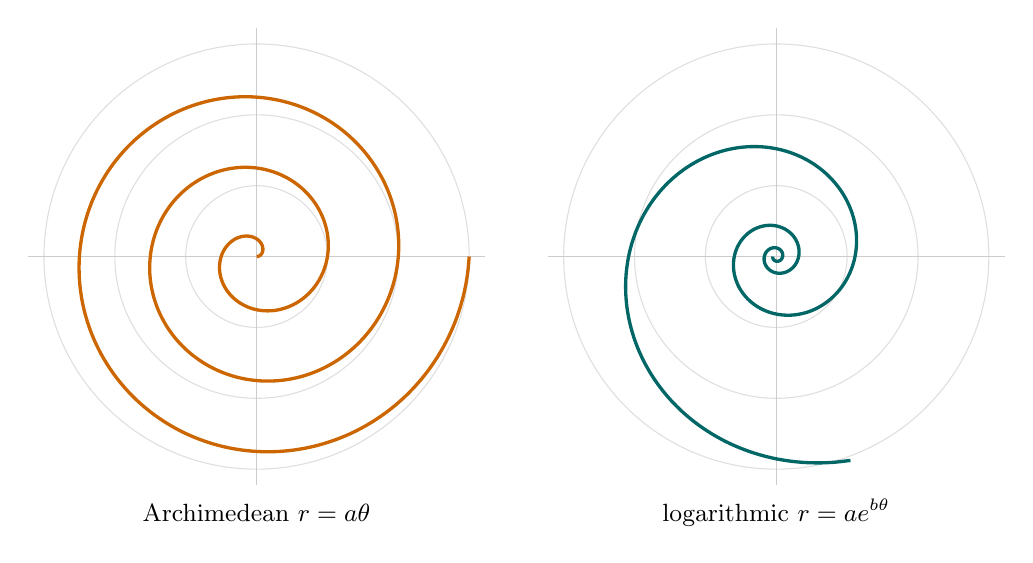
\begin{tikzpicture}
  \begin{scope}
    \foreach \r in {1,2,3} { \draw[gray!25] (0,0) circle (\r*0.9); }
    \draw[gray!40] (-2.9,0) -- (2.9,0) (0,-2.9) -- (0,2.9);
    \draw[very thick, orange!80!black, domain=0:1080, samples=300, smooth, variable=\t]
      plot ({\t/400*cos(\t)}, {\t/400*sin(\t)});
    \node[font=\small] at (0,-3.25) {Archimedean $r = a\theta$};
  \end{scope}
  \begin{scope}[xshift=6.6cm]
    \foreach \r in {1,2,3} { \draw[gray!25] (0,0) circle (\r*0.9); }
    \draw[gray!40] (-2.9,0) -- (2.9,0) (0,-2.9) -- (0,2.9);
    \draw[very thick, teal!80!black, domain=-900:290, samples=300, smooth, variable=\t]
      plot ({1.0*exp(0.0035*\t)*cos(\t)}, {1.0*exp(0.0035*\t)*sin(\t)});
    \node[font=\small] at (0,-3.25) {logarithmic $r = a e^{b\theta}$};
  \end{scope}
\end{tikzpicture}
